\documentclass[aspectratio=169]{beamer}


\mode<presentation>
{
  \usetheme{Madrid}%\usetheme{uzhneu-en}
  \setbeamercovered{transparent}
  %\usecolortheme{crane}
\usefonttheme{professionalfonts}

}
\setbeamertemplate{navigation symbols}{}

%\usepackage[numbers]{natbib}
\usepackage{graphicx} %include i grafici
\graphicspath{{pictures/img/}}
\usepackage[english]{babel}
\usepackage[normal]{subfigure}

\usepackage{amsthm}
\usepackage{amssymb}
\usepackage{amsmath}
\usepackage{cancel}
\usepackage{comment}
%\DeclareMathOperator{\supp}{supp}
\usepackage{mathrsfs}
\usepackage{latexsym}
\usepackage{graphicx}
\DeclareGraphicsExtensions{.pdf,.jpg}
\usepackage{subfigure}
\usepackage{hyperref}
%\hypersetup{colorlinks=true,linkcolor=blue}
\usepackage{amsfonts}
\usepackage{bm}
\usepackage{algorithm2e}

\usepackage[style=authortitle,backend=bibtex]{biblatex}
%\bibliography{biblio}

\usepackage[utf8]{inputenc}

\usepackage{tikz}

\usepackage{bbm}
\usepackage{times}
\usepackage[T1]{fontenc}


\newtheorem{induction_hyp}{Induction Hypothesis}
\newtheorem{remark}{Remark}
\newtheorem{algo}{Algorithm}

\definecolor{green}{rgb}{0.0, 0.42, 0.14}

\newcommand{\R}{\mathbb R}
\newcommand{\Z}{\mathbb Z}
\newcommand{\N}{\mathbb N}
\newcommand{\C}{\mathbb C}
\newcommand{\Q}{\mathbb Q}
\newcommand{\K}{\mathbb K}
\newcommand{\PP}{\mathbb P}
\newcommand{\TT}{\mathcal{T}}
\newcommand{\normal}{\mathbf{N}}

\renewcommand{\SS}{\mathcal{S}}
\newcommand{\KK}{\mathcal{K}}
\newcommand{\EE}{\mathcal{E}}

%%%%%Dante 
\newcommand{\diff}[1]{{\mathrm{d}{#1}}}
\newcommand{\dotprod}{\boldsymbol \cdot}
\newcommand{\ddt}[1]   {\frac{\partial{#1}}{\partial{t}}}
\newcommand{\dsddt}[1] {\dfrac{\partial{#1}}{\partial{t}}}
\newcommand{\txddt}[1] {\tfrac{\partial{#1}}{\partial{t}}}
\newcommand{\ddp}[2]   { \frac{\partial #1}{\partial #2}}
\newcommand{\dsddp}[2] {\dfrac{\partial #1}{\partial #2}}
\newcommand{\txddp}[2] {\tfrac{\partial #1}{\partial #2}}
\newcommand{\ddo}[2]   { \frac{\diff #1}{\diff #2}}
\newcommand{\dsdo}[2]  {\dfrac{\diff #1}{\diff #2}}
\newcommand{\txddo}[2] {\tfrac{\diff #1}{\diff #2}}
\newcommand{\Div}[1] { \boldsymbol{\nabla} \!\dotprod #1 }
\newcommand{\Grad}[1] { \boldsymbol{\nabla} #1 }
\newcommand{\Gradr}[1]{\widetilde{\boldsymbol{\nabla} {#1}}}
\newcommand{\vect}[1] {\ww{#1}}
\newcommand{\versor}[1] {\hat{ \boldsymbol{#1}}}
\newcommand{\vzero}{\boldsymbol{0}}
\newcommand{\IdxM} {\mathbb{I}}

 %----------------> Euler and NS equation
\newcommand{\vel}{\boldsymbol{v}}
\newcommand{\mm}{\boldsymbol{m}}
%\newcommand{\ee}{e}
\newcommand{\hh}{h}
\newcommand{\Et}{E^t}
\newcommand{\et}{e^t}
\newcommand{\qq}{\vect{q}}
\newcommand{\Rgas}{\mathcal{R}}
\newcommand{\vecu}{\mathsf{u}}
\newcommand{\vecf}{\boldsymbol{\mathsf{f}}}
\newcommand{\vecfa}{\boldsymbol{\mathsf{f}}^a}
\newcommand{\vecfv}{\boldsymbol{\mathsf{f}}^v}
\newcommand{\Jac}{\boldsymbol{\mathsf{A}}}   
\newcommand{\viscT}{\mathbb{S}}
\newcommand{\Kgas}{\kappa}

 %---------------> Numerical scheme
%\newcommand{\Rese}{{{\Phi}^e}}
%\newcommand{\Resei}{{{\Phi}^e_i}}
%\newcommand{\Reseib}{{{\Phi}^{f,\,\scriptscriptstyle{\partial}}_i}}
%\newcommand{\HResei}{{{\hat{\Phi}}^e_i}}
%\newcommand{\sHResei}{{{\hat{\Phi}}^{\,e, \star}_i}}
%\newcommand{\LResei}{{{\tilde{\Phi}}^e_i}}
%\newcommand{\vecw}{\mathsf{w}}
\newcommand{\ResKs}{{{\Phi}^K_\sigma}}
\newcommand{\ResK}{{{\Phi}^K}}
        
%---------------> Text style
\newcommand{\Tr}{\mathrm{T}}
\newcommand{\diag}{\mathop{\mathrm{diag}}}
\newcommand{\xx}{\boldsymbol{x}}
\newcommand{\dV}{\,\mathrm{d}\Omega}
\newcommand{\dS}{\,\mathrm{d}\partial\Omega}
\newcommand{\vecn}{\boldsymbol{\mathbf n}}
\newcommand{\Ndofe}{N^e_\mathrm{dof}}
\newcommand{\Ndim}{{N_\mathrm{dim}}}
\newcommand{\Neqn}{{N_\mathrm{eq}}}
\newcommand{\E}{\mathrm{E}}
\newcommand{\FF}{\boldsymbol{\mathsf{R}}} 
\newcommand{\JJ}{\mathbb{J}} 
\newcommand{\bbf}{{\mathbf {f}}}
\newcommand{\bxx}{{\mathbf {x}}}
\newcommand{\bn}{{\mathbf {n}}}
\newcommand{\s}{\sqrt{2}}
\newcommand{\is}{\frac{\sqrt{2}}{2}}
\newcommand{\hf}{\hat{f}}

\newcommand{\dpar}[2]{\dfrac{\partial #1}{\partial #2}}
\newcommand{\bu}{\mathbf{u}}
\newcommand{\bv}{\mathbf{v}}
\newcommand{\Bv}{\underline{\mathbf{v}}}
\newcommand{\bbv}{\mathbf{v}}
\newcommand{\Bbv}{\underline{\mathbf{v}}}
\newcommand{\bF}{\mathbf{F}}
\newcommand{\bFF}{\mathcal{F}}
\newcommand{\bbF}{\mathbf{\mathcal{F}}}
\newcommand{\bK}{\mathbf{K}}
\newcommand{\bbu}{\mathbf{u}}
\newcommand{\bbg}{\mathbf{g}}
\newcommand{\hbbg}{\hat{\mathbf{g}}}
\newcommand{\hbbf}{\hat{\mathbf{f}}}
\newcommand{\hbbfe}{\hat{\mathbf{f}}_{\sigma,\sigma'}}
\newcommand{\ba}{\mathbf{a}}
\newcommand{\bx}{\mathbf{x}}
\newcommand{\by}{\mathbf{y}}
\newcommand{\red}[1]{\textcolor{red}{#1}}
\newcommand{\blue}[1]{\textcolor{blue}{#1}}
\newcommand{\ICI}{\red{\large{ICI}}}

% ---- Notation Philipp
\newcommand{\ww}[1]{\underline{#1}}
\renewcommand{\div}{\operatorname{div}}
\newcommand{\est}[1]{\left\langle#1\right\rangle}
\newcommand{\bU}{\mathbf{U}}
\newcommand{\bH}{\mathbf{H}}
\newcommand{\dd}{\mathrm{d}}
\newcommand{\bV}{\mathbf{V}}
\newcommand{\mean}[1]{\overline{#1}}
\newcommand{\bbfh}{{\mathbf {f}^h}}
\newcommand{\Ol}{\mathcal{O}}
\newcommand{\WW}{\mathrm{W}}
\newcommand{\LL}{\mathcal{L}}
\newcommand{\II}{\hat{I}_0}
\newcommand{\1}{\begin{pmatrix}
                 1\\
                 1
                \end{pmatrix}}
\newcommand{\e}[1]{\mathrm{e^{#1}}}
\newcommand{\VV}{\mathcal{V}}
\newcommand{\gnum}{g^{\operatorname{num}}}

\newcommand\norm[1]{\left\lVert#1\right\rVert}

%Numerical schemes
\newcommand{\Resjr}{\Phi^{j+\frac{1}{2}}_j}
\newcommand{\Resjl}{\Phi^{j-\frac{1}{2}}_j}

\newcommand{\Resjrn}{\Phi^{j+\frac{1}{2},n}_j}
\newcommand{\Resjln}{\Phi^{j-\frac{1}{2},n}_j}


\newcommand{\cc}[1]{\chi_{[t^0,t^{#1}]}}



%\newcommand{\L}{\mathcal{L}}


\renewcommand{\vec}[1]{\ww{#1}}
\newcommand{\mat}[1]{\ww{\ww{#1}}}
%Davide

\def\STC{T^n\times V_i}
\def\SC{V_i}
\def\TC{T^n}
\def\L{\mathcal{L}}
\def\I{\mathcal{I}}
\def\R{\mathbb{R}}
\def\dt{\Delta t}
\newcommand{\matz}{\underline{\underline{0}}}
\def\bbc{\underline{\boldsymbol{u}}}
\def\bc{\boldsymbol{u}}
\def\br{\boldsymbol{r}}
\def\bd{\mathbf{d}}
\def\bbd{\underline{\mathbf{d}}}
\def\bphi{\underline{\phi}}
\def\M{\underline{\underline{\mathrm{M}}}}
\def\RHS{\underline{\underline{\mathrm{R}}}}
\def\bE{F}
\def\bG{F}
\newcommand{\uvec}[1]{\ww{#1}}
\def\vecbeta{\ww{\beta}}
\def\vecz{\ww{0}}
\def\matz{\ww{\ww{0}}}
%Colors 
\definecolor{darkspringgreen}{rgb}{0., 0.55, 0.3}
\definecolor{dartmouthgreen}{rgb}{0.05, 0.5, 0.06}
\definecolor{etonblue}{rgb}{0.59, 0.78, 0.64}
\definecolor{airforceblue}{rgb}{0., 0.4, 0.66}
\definecolor{arylideyellow}{rgb}{0.91, 0.84, 0.42}
\definecolor{emerald}{rgb}{0.31, 0.78, 0.47}
\definecolor{uclagold}{rgb}{1.0, 0.7, 0.0}
\definecolor{cadmiumorange}{rgb}{0.93, 0.53, 0.18}




% Evidenziato
\newcommand{\TODO}[1]{{\color{red}#1}}
\newcommand{\highlight}[1]{\textbf{\color{bluemathlab}#1}}
\newcommand{\highlightB}[1]{\textbf{\color{black!15!orangemathlab}#1}}
\newcommand{\mathhighlight}[1]{\color{bluemathlab}#1}
\newcommand{\mathhighlightB}[1]{\color{black!15!orangemathlab}#1}

% Framebreaks: move continuation count from subtitle to title
\setbeamertemplate{frametitle continuation}[from second][]
\makeatletter 
\long\def\beamer@@frametitle[#1]#2{% 
	\beamer@ifempty{#2}{}{% 
		\gdef\insertframetitle{#2\ifnum\beamer@autobreakcount>1\relax{}\space(\insertcontinuationcountroman)\fi}% 
		\gdef\beamer@frametitle{#2}% 
		\gdef\beamer@shortframetitle{#1}% 
	}% 
}
\makeatother 

\setbeamercolor{blockcolor1}{fg=black,bg=bluemathlab!10}
\setbeamercolor{blockcolor2}{fg=black,bg=orangemathlab!10} 
\title[ADER vs DeC]{ADER and DeC: \\ arbitrarily high order (explicit)\\ methods for PDEs and ODEs} 

\author[D. Torlo]{Davide Torlo}

\institute[Inria]
{Inria Bordeaux - Sud Ouest\\
Team Cardamom}


\date[]
{\small Based on: Han Veiga, M., Öffner, P. \& Torlo, D. \textit{DeC and ADER: Similarities, Differences and a Unified Framework.} J Sci Comput 87, 2 (2021). https://doi.org/10.1007/s10915-020-01397-5
}


\AtBeginSection[]
{
	\begin{frame}<beamer>
	\frametitle{Outline}
	  \tableofcontents[currentsection]
  
	\end{frame}


}

\begin{document}

\begin{frame}

\titlepage



\end{frame}

\begin{frame}<beamer>
	\frametitle{Outline}
	  \tableofcontents
  % You might wish to add the option [pausesections]
\end{frame}

\section{Motivation}

\begin{frame}{Motivation: high order accurate explicit method}
	We want to solve a hyperbolic  PDE system for $u:\R^+\times \Omega \to \R^D$
	\begin{equation}\label{eq:scalarPDE}
		\partial_t u + \nabla_{\mathbf{x}} \mathcal{F}(u) =0.
	\end{equation}

	Or ODE system for $\bc:\R^+\to \R^S$
	\begin{equation}\label{eq:scalarODE}
		\partial_t \bc + F(\bc) =0.
	\end{equation}
	
	Applications:
	\begin{itemize}
		\item Fluids/transport
		\item Chemical/biological processes
	\end{itemize}
	\vspace{5mm}
	
	How?
	\begin{itemize}
		\item Arbitrarily high order accurate
		\item \only<3>{Explicit (if nonstiff problem)}
	\end{itemize}
	
	\only<2>{
		\begin{tikzpicture}[remember picture,overlay]
			\node at (current page.center) {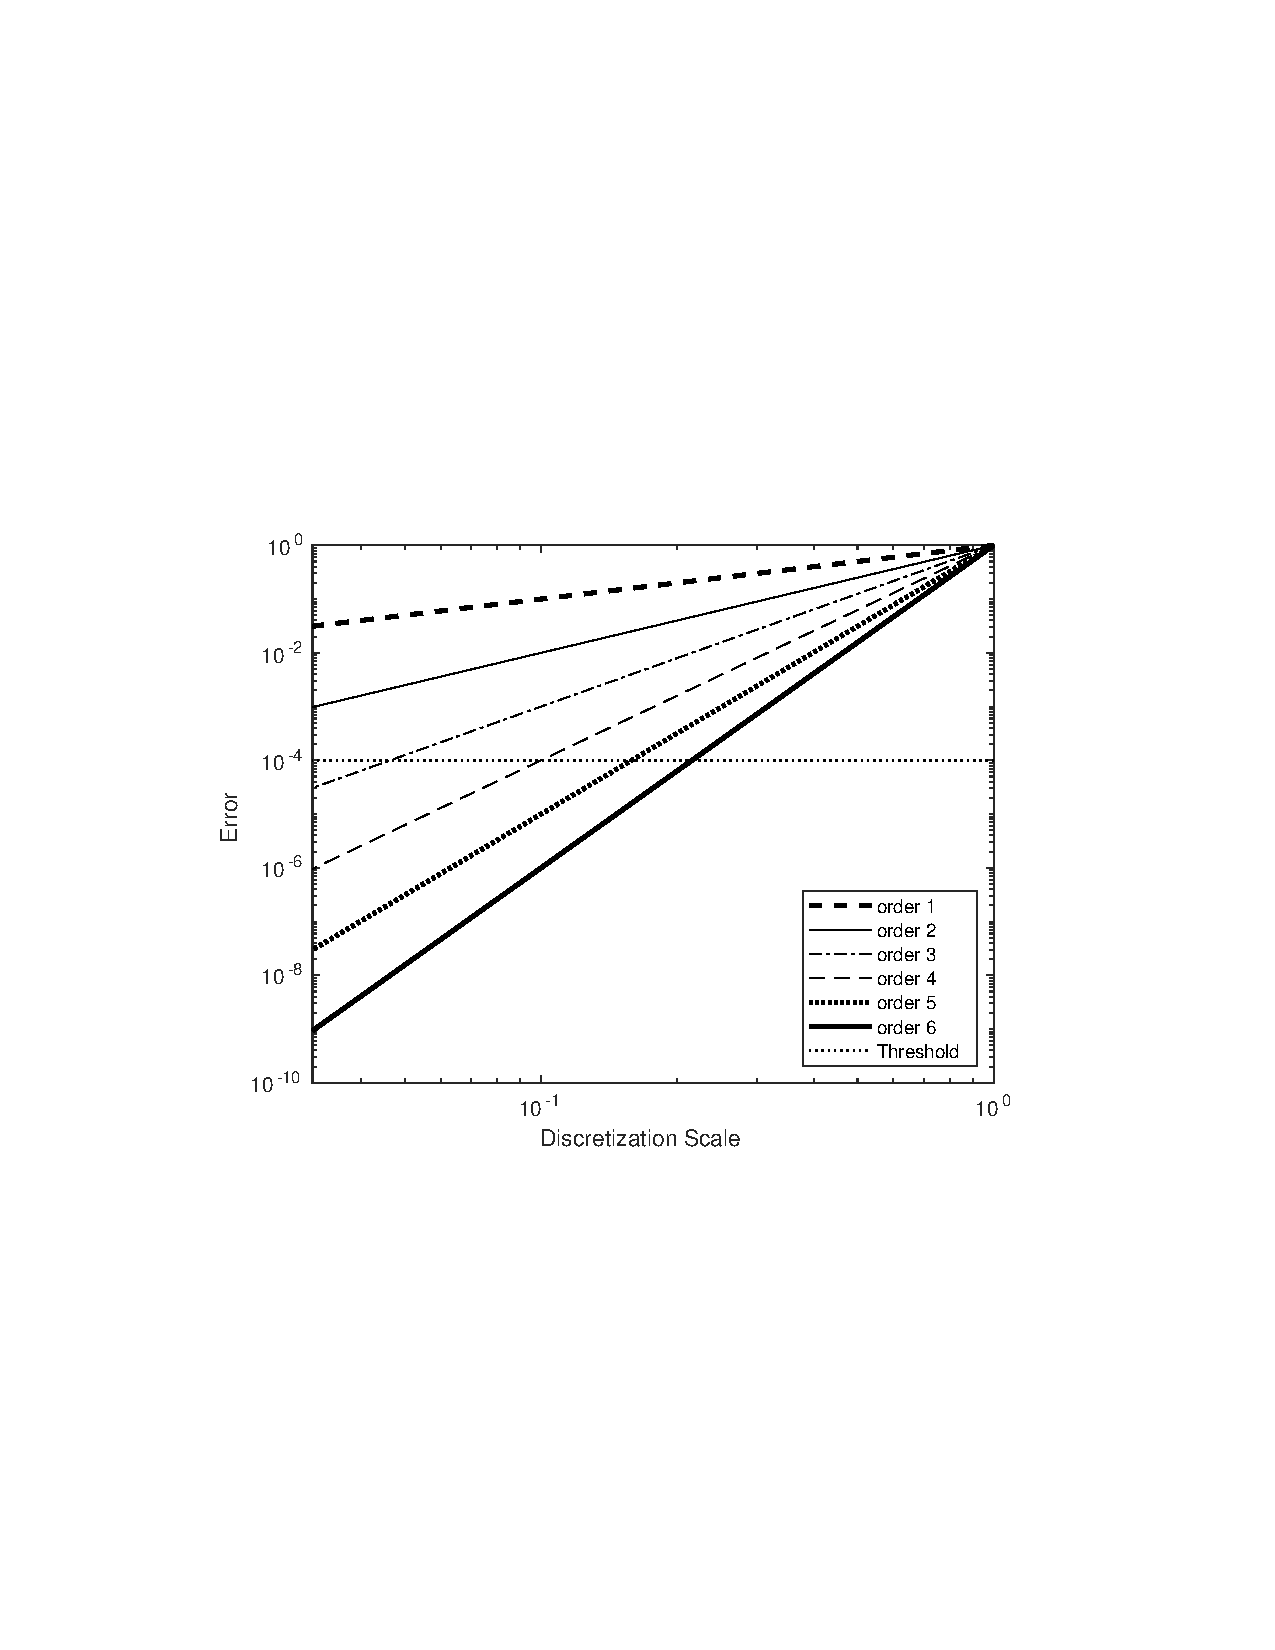
\includegraphics[width=0.81\textwidth]{pictures/HighOrderMethods.pdf}};
		\end{tikzpicture}
	}
	
\end{frame}




\begin{frame}{Classical time integration: Runge--Kutta}
\begin{align}
	&\bc^{(1)}:=\bc^n,\\
	&\bc^{(k)}:=\bc^n+\sum_{s=1}^{K} A_{ks} F\left(t^n+b_s\Delta t,\bc^{(s)}\right), \quad \text{for } k=2,\dots, K, \label{eq:RK}\\
	&\bc^{n+1}:= \sum_{k=1}^K \gamma_k \bc^{(k)}.
\end{align}
 
\end{frame}

\begin{frame}{Classical time integration: Explicit Runge--Kutta}
\begin{align*}
	&\bc^{(k)}:=\bc^n+\sum_{s=1}^{k-1} A_{ks} F\left(t^n+b_s\Delta t,\bc^{(s)}\right), \quad \text{for } k=2,\dots, K.
\end{align*}

\begin{itemize}
\item Easy to solve
\item High orders involved:
\begin{itemize}
\item Order conditions: system of many equations
\item Stages  $K\geq d$ order of accuracy (e.g. RK44, RK65) 
\end{itemize}
\end{itemize} 
 
\end{frame}

\begin{frame}{Classical time integration: Implicit Runge--Kutta}
\begin{align*}
	&\bc^{(k)}:=\bc^n+\sum_{s=1}^{K} A_{ks} F\left(t^n+b_s\Delta t,\bc^{(s)}\right), \quad \text{for } k=2,\dots, K.
\end{align*}

\begin{itemize}
\item More complicated to solve for nonlinear systems
\item High orders easily done:
\begin{itemize}
\item Take a high order quadrature rule on $[t^n,t^{n+1}]$
\item Compute the coefficients accordingly, see Gauss--Legendre or Gauss--Lobatto polynomials
\item Order up to $d=2K-1$ 
\end{itemize}
\end{itemize} 
 
\end{frame}

\begin{frame}{ADER and DeC}
Two iterative explicit arbitrarily high order accurate methods.
\begin{itemize}
\item ADER\footnote{M. Dumbser, D. S. Balsara, E. F. Toro, and C.-D. Munz. A unified framework for the construction of one-step finite volume and discontinuous galerkin schemes on unstructured meshes. Journal of Computational Physics, 227(18):8209–8253, 2008.} for hyperbolic PDE, after a first analytic more complicated approach.
\item Deferred Correction (DeC): introduced for explicit ODE\footnote{A. Dutt, L. Greengard, and V. Rokhlin. Spectral Deferred Correction Methods for Ordinary Differential Equations. BIT Numerical Mathematics, 40(2):241–266, 2000.}, extended to implicit ODE\footnote{M. L. Minion. Semi-implicit spectral deferred correction methods for ordinary differential equations. Commun. Math. Sci., 1(3):471–500, 09 2003.} and to hyperbolic PDE\footnote{R. Abgrall. High order schemes for hyperbolic problems using globally continuous approximation and avoiding mass matrices. Journal of Scientific Computing, 73(2):461–494, Dec 2017.}.
\end{itemize}
\end{frame}

\section{DeC}
\begin{frame}{DeC high order time discretization: $\L^2$}
	\begin{minipage}{0.65\textwidth}
	High order in time: we discretize our variable on $[t^n, t^{n+1}]$ in $M$ substeps ($\bc^{m}$).
		\begin{equation*}
			\partial_t\bc + F(\bc(t))=0.
		\end{equation*}
	
		Thanks to Picard–Lindelöf theorem, we can rewrite 	\begin{equation*}
			\bc^{m}=\bc^0 -\int_{t^0}^{t^m} F(\bc(t))dt.
		\end{equation*} and if we want to reach order $r+1$ we need $M=r$. 
	\end{minipage}
	\begin{minipage}{0.32\textwidth}
		\begin{figure}[h]
			\centering
			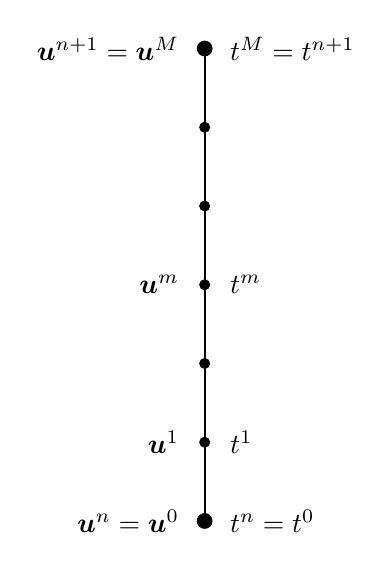
\begin{tikzpicture}
				\draw [thick]   (0,0) -- (0,6) node [right=2mm]{};
				% nodes
				\fill[black]    (0,0) circle (1mm) node[right=2mm] {$t^n=t^0$} node[left=2mm] {$\bc^{n}=\bc^0$} 
				(0,1) circle (0.7mm) node[right=2mm] {$t^1$} node[left=2mm] {$\bc^1$} 
				(0,2) circle (0.7mm) node[right=2mm] {}
				(0,3) circle (0.7mm) node[right=2mm] {$t^m$ } node[left=2mm] {$\bc^m$} 
				(0,4) circle (0.7mm) node[right=2mm] {}
				(0,5) circle (0.7mm) node[right=2mm] {}
				(0,6) circle (1mm) node[right=2mm] {$t^M=t^{n+1}$} node[left=2mm] {$\bc^{n+1}=\bc^M$} ;
			\end{tikzpicture}
		\end{figure}
	\end{minipage}
	
\end{frame}



\begin{frame}{DeC high order time discretization: $\L^2$}
	\begin{minipage}{0.77\textwidth}
		More precisely, for each $\sigma$ we want to solve $\L^2 (\bc^{n,0},\dots,\bc^{n,M})=0$, where 
		{\begin{align*}
			\L^2(\bc^0, \dots, \bc^M) &
			\only<1>{=
			\begin{pmatrix}
				\bc^M-\bc^0 -\sum_{r=0}^M \int_{t^0}^{t^M} F(\bc^r) \varphi_r(s) \diff s\\
				\vdots\\
				\bc^1-\bc^0 - \sum_{r=0}^M \int_{t^0}^{t^1} F(\bc^r) \varphi_r(s) \diff s
			\end{pmatrix}
		}
			\only<2>{=
			\begin{pmatrix}
				\bc^M-\bc^0 -\Delta t \sum_{r=0}^M \theta_r^M F(\bc^r) \\
				\vdots\\
				\bc^1-\bc^0 - \Delta t \sum_{r=0}^M  \theta_r^1  F(\bc^r) 
			\end{pmatrix}}
		\end{align*}
	}
		\begin{itemize}
			\item $\L^2=0$ is a system of $M \times S$ coupled (non)linear equations
			\item $\L^2$ is an implicit method 
			\item Not easy to solve directly $\L^2(\bbc^*)=0$
			\item High order ($\geq M+1$), depending on points distribution
		\end{itemize}
		
	\end{minipage}\hfill
	\begin{minipage}{0.2\textwidth}
		\begin{figure}[h]
			\centering
			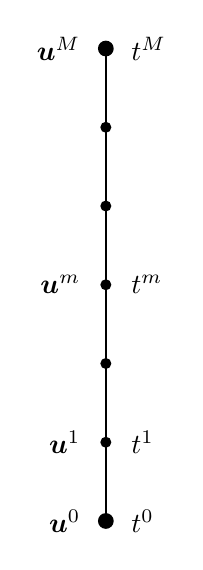
\begin{tikzpicture}
				\draw [thick]   (0,0) -- (0,6) node [right=2mm]{};
				% nodes
				\fill[black]    (0,0) circle (1mm) node[right=2mm] {$t^{0}$} node[left=2mm] {$\bc^{0}$} 
				(0,1) circle (0.7mm) node[right=2mm] {$t^{1}$} node[left=2mm] {$\bc^{1}$} 
				(0,2) circle (0.7mm) node[right=2mm] {}
				(0,3) circle (0.7mm) node[right=2mm] {$t^{m}$ } node[left=2mm] {$\bc^{m}$} 
				(0,4) circle (0.7mm) node[right=2mm] {}
				(0,5) circle (0.7mm) node[right=2mm] {}
				(0,6) circle (1mm) node[right=2mm] {$t^{M}$} node[left=2mm] {$\bc^{M}$} ;
			\end{tikzpicture}
		\end{figure}
	\end{minipage}
\end{frame}

\begin{frame}{DeC low order time discretization: $\L^1$}
	\begin{minipage}{0.77\textwidth}
		Instead of solving the implicit system directly (difficult), we introduce a first order scheme $\L^1(\bc^{n,0},\dots,\bc^{n,M})$:
		\begin{align*}
			&\L^1(\bc^{0},\dots,\bc^{M})=
			\begin{pmatrix}
				\bc^M-\bc^0 -\Delta t \beta^M F(\bc^0) \\
				\vdots\\
				\bc^1-\bc^0 - \Delta t \beta^1  F(\bc^0) 
			\end{pmatrix}
		\end{align*}
		\begin{itemize}
			\item First order approximation
			\item Explicit Euler
			\item Easy to solve $\L^1(\bbc)=0$
		\end{itemize}
	\end{minipage}\hfill
	\begin{minipage}{0.2\textwidth}
		\begin{figure}[h]
			\centering
			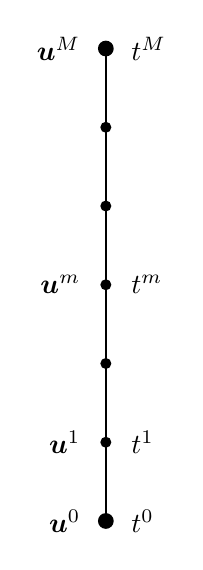
\begin{tikzpicture}
	\draw [thick]   (0,0) -- (0,6) node [right=2mm]{};
	% nodes
	\fill[black]    (0,0) circle (1mm) node[right=2mm] {$t^{0}$} node[left=2mm] {$\bc^{0}$} 
	(0,1) circle (0.7mm) node[right=2mm] {$t^{1}$} node[left=2mm] {$\bc^{1}$} 
	(0,2) circle (0.7mm) node[right=2mm] {}
	(0,3) circle (0.7mm) node[right=2mm] {$t^{m}$ } node[left=2mm] {$\bc^{m}$} 
	(0,4) circle (0.7mm) node[right=2mm] {}
	(0,5) circle (0.7mm) node[right=2mm] {}
	(0,6) circle (1mm) node[right=2mm] {$t^{M}$} node[left=2mm] {$\bc^{M}$} ;
\end{tikzpicture}
		\end{figure}
	\end{minipage}
\end{frame}
\begin{comment}
\begin{frame}{DeC: Iterative process}
	$K$ iterations where the iteration index is the superscript $(k)$, with $k=0,\dots, K$
	\begin{enumerate}
		\item Define $\bc^{(0),m}=\bc^n=\bc(t^n)$ for $m=0,\dots,M$
		\item Define $\bc^{(k),0}=\bc(t^n)$ for $k=0,\dots,K$
		\item Find $\bbc^{(k)}$ as $\L^1(\bbc^{(k)})=\L^1(\bbc^{(k-1)})-\L^2(\bbc^{(k-1)})$
		\item $\bc^{n+1}= \bc^{(K),M}$.
	\end{enumerate}
	
	\begin{theorem}[Convergence DeC]
		\begin{itemize}
			\item If $\L^1$ coercive with constant $C_1$
			\item If $\L^1-\L^2$ Lipschitz with constant $C_2 \Delta t$
		\end{itemize}
		Then $\lVert \bbc^{(k)}-\bbc^*\rVert \leq C\Delta t^k$
	\end{theorem}
	Hence, choosing $K=M+1$, then $\lVert \bc^{(K),M}-\bc^{ex}(t^{n+1})\rVert \leq C\Delta t ^K$
\end{frame}
\end{comment}
\begin{frame}{Deferred Correction\footnote{A. Dutt, L. Greengard, and V. Rokhlin. BIT Numerical Mathematics, 40(2):241–266,
			2000.}}
	How to combine two methods keeping the accuracy of the second and the stability and simplicity of the first one?
	
	\begin{minipage}{0.58\textwidth}
		\begin{equation*}\label{DeC_method}
			\begin{split}
				&\bc^{0,(k)}:=\bc(t^n), \quad k=0,\dots, K,\\
				&\bc^{m,(0)}:=\bc(t^n),\quad m=1,\dots, M\\
				&\L^1(\bbc^{(k)})=\L^1(\bbc^{(k-1)})-\L^2(\bbc^{(k-1)})\text{ with }k=1,\dots,K.
			\end{split}
		\end{equation*}\vspace{-4mm}
\begin{theorem}[Convergence DeC]
	\begin{itemize}
		\item $\L^2(\bbc^*)=0$
		\item If $\L^1$ coercive with constant $C_1$
		\item If $\L^1-\L^2$ Lipschitz with constant $C_2 \Delta t$
	\end{itemize}
	Then $\lVert \bbc^{(K)}-\bbc^*\rVert \leq C(\Delta t)^K$
\end{theorem}
	\end{minipage} \hfill
	\begin{minipage}{0.4\textwidth}
		\begin{itemize}
			{
				\item $\mathcal{L}^1(\bbc)=0$, first order accuracy, easily invertible.
				\item $\mathcal{L}^2(\bbc)=0$, high order $M+1$.
			}
		\end{itemize}
		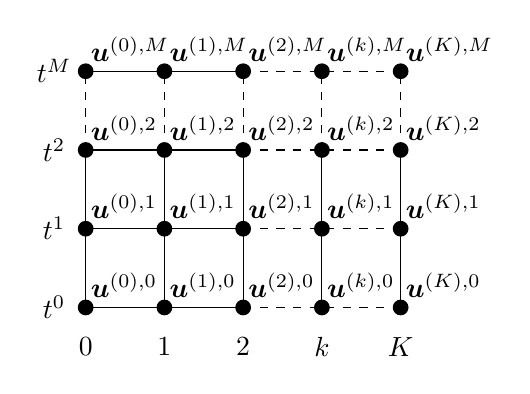
\begin{tikzpicture}
			\tikzset{dot/.style={fill=black,circle}}
			
			\foreach\l[count=\y] in {0,1,2,M}
			{
				\draw (1,\y) -- (3,\y);
				\draw[dashed] (3,\y) -- (5,\y);
				\node at (0.6,\y){$t^{\l}$};
				\foreach\foreach\z[count=\x] in {0,1,2,k,K}
				{
					\only<\x>{\fill (\x,\y) circle (1mm) node[anchor=south west] {$\!\bc^{(\z),\l}$};}
				}
			}
			
			\foreach\l[count=\x] in {0,1,2,k,K}
			{
				\draw (\x,1) -- (\x,3);
				\draw[dashed] (\x,3) -- (\x,4);
				\node at (\x,0.5){$\l$};
			}
			
		\end{tikzpicture}
	\end{minipage}
	
\end{frame}
%\begin{frame}{Deferred Correction\footnote{A. Dutt, L. Greengard, and V. Rokhlin. Spectral Deferred Correction Methods
%			for Ordinary Differential Equations. BIT Numerical Mathematics, 40(2):241–266,
%			2000.}}
%	How to combine two methods keeping the accuracy of the second and the stability and simplicity of the first one?\\
%	\begin{itemize}
%		{
%			\item $\mathcal{L}^1(f^{n+1},f^n)=0$, first order accuracy, easily invertible (IMEX).
%			\item $\mathcal{L}^2(f^{n+1},f^n)=0$, high order $r$ (>1), not directly solvable.
%		}
%	\end{itemize}
%	\pause
%	\begin{algo}[DeC method]
%		\begin{itemize}
%			\item $\mathcal{L}^1(f^{(1)},f^n)=0$, prediction $f^{(1)}$.
%			\item For $j=2,\dots,K$ corrections: \\ $\quad \mathcal{L}^1(f^{(j)},f^n)=\mathcal{L}^1(f^{(j-1)},f^n)-\mathcal{L}^2(f^{(j-1)},f^n).$
%			\item $f^{n+1}:=f^{(K)}$.
%		\end{itemize}
%	\end{algo}
%	\begin{remark}
%		$\mathcal{L}^1$ is used implicitly and $\mathcal{L}^2$ only explicitly.
%	\end{remark}
%\end{frame}

%\begin{frame}{Deferred Correction}
%			\begin{theorem}[Deferred Correction convergence]
%		Given the DeC procedure. If
%		\begin{itemize}
%			\item $\mathcal{L}^1$ is coercive with constant $\alpha_1$
%			\item $\mathcal{L}^2-\mathcal{L}^1$ is Lipschitz continuous with constant $\alpha_2 \Delta$
%			\item $\exists !\, f^{*}_\Delta$ such that $\mathcal{L}^2(f^{*}_\Delta)=0$.
%		\end{itemize}
%		Then if $\eta=\frac{\alpha_2}{\alpha_1}\Delta<1$, the deferred correction is converging to $ f^*_\Delta$ and after $K$ iterations the error is smaller than $\eta^K$ times the original error.
%	\end{theorem}
%\end{frame}

\begin{frame}{DeC -- Proof}
	
	\small
	\begin{proof}
		Let $f^*$ be the solution of $\L^2(\bbc^*)=0$. We know that $\L^1(\bbc^*)=\L^1(\bbc^*)-\L^2(\bbc^*)$, so that
		\visible<2>{
		\begin{align*}
			\L^1(\bbc^{(k+1)})-\L^1(\bbc^*)=&\left(\L^1(\bbc^{(k)})-\L^2(\bbc^{(k)})\right)-\left(\L^1(\bbc^*)-\L^2(\bbc^*)\right)  \\
			{\color{red}C_1 }||\bbc^{(k+1)}-\bbc^*||\leq & ||\L^1(\bbc^{(k+1)})-\L^1(\bbc^*)||=\\
			=&||\L^1(\bbc^{(k)})-\L^2(\bbc^{(k)})-(\L^1(\bbc^*)-\L^2(\bbc^*))||\leq \\
			\leq &  {\color{red} C_2 \Delta } ||\bbc^{(k)}-\bbc^*||.\\
			||\bbc^{(k+1)}-\bbc^*||\leq &\left(\frac{C_2}{C_1}\Delta\right) ||\bbc^{(k)}-\bbc^*|| \leq \left(\frac{C_2}{C_1}\Delta\right)^{k+1} ||\bbc^{(0)}-\bbc^*||.
		\end{align*}
		After $K$ iteration we have an error at most of $\left(\frac{C_2}{C_1}\Delta\right)^K ||\bbc^{(0)}-\bbc^*||$. }
	\end{proof}
	
\end{frame}



\begin{comment}
\begin{frame}{DeC: $\L^2$ operator}
\begin{align*}
\L^2(\bc^0, \dots, \bc^M) &=
\begin{cases}
 \bc^M-\bc^0 -\int_{t^0}^{t^M} \I_M ( F(\bc^0),\dots,F(\bc^M))ds
\\
\dots\\
\bc^1-\bc^0 - \int_{t^0}^{t^1} \I_M ( F(\bc^0),\dots,F(\bc^M))ds
\end{cases}\\
 &=
\begin{cases}
\bc^M-\bc^0 -\sum_{r=0}^M \int_{t^0}^{t^M} F(\bc^r) \varphi_r(s) \diff s\\
\dots\\
\bc^1-\bc^0 - \sum_{r=0}^M \int_{t^0}^{t^1} F(\bc^r) \varphi_r(s) \diff s
\end{cases}
\\
 &=
\begin{cases}
\bc^M-\bc^0 -\Delta t \sum_{r=0}^M \theta_r^M F(\bc^r) \\
\dots\\
\bc^1-\bc^0 - \Delta t \sum_{r=0}^M  \theta_r^1  F(\bc^r) 
\end{cases}
\end{align*}

\end{frame}

\begin{frame}{DeC: $\L^2$ operator}
Goal: find $\bbc^*=(\bc^0, \dots, \bc^m, \dots, \bc^M)^*$ : $\L^2(\bbc^*)=0$.
\vspace{1cm}
\begin{itemize}
\item $\L^2=0$ is a system of $M \times S$ coupled (non)linear equations
\item $\L^2$ is an implicit method 
\item Not easy to solve directly
\item High order ($\geq M+1$), depending on points distribution
\end{itemize}
\end{frame}
\begin{frame}{DeC: $\L^1$ operator}
\begin{equation}\label{eq:L1}
\L^1(\bc^0, \dots, \bc^M) :=
\begin{cases}
 \bc^M-\bc^0 - \beta^M \Delta t F(\bc^0) \\
\vdots\\
\bc^1- \bc^0 - \beta^1 \Delta t F(\bc^0)
\end{cases} \quad\beta^m:=\frac{t^m-t^0}{t^M-t^0}. 
\end{equation}
\begin{itemize}
\item First order approximation
\item Explicit Euler
\item Easy to solve $\L^1(\bbc)=0$
\end{itemize}
\end{frame}

%
\end{comment}

\begin{comment}
\begin{frame}{DeC -- Proof}
\small
\begin{proof}
Let $\bbc^*$ be the solution of $\L^2(\bbc^*)=0$. We know that $\L^1(\bbc^*)=\L^1(\bbc^*)-\L^2(\bbc^*)$ and $\L^1(\bbc^{(k+1)})=\left(\L^1(\bbc^{(k)})-\L^2(\bbc^{(k)})\right)$, so that
\begin{align*}
C_1 ||\bbc^{(k+1)}-\bbc^*||\leq & ||\L^1(\bbc^{(k+1)})-\L^1(\bbc^*)||=\\
=&||\L^1(\bbc^{(k)})-\L^2(\bbc^{(k)})-(\L^1(\bbc^*)-\L^2(\bbc^*))||\leq \\
\leq &  C_2 \Delta t ||\bbc^{(k)}-\bbc^*||.\\
||\bbc^{(k+1)}-\bbc^*||\leq &\left(\frac{C_2}{C_1}\Delta t\right) ||\bbc^{(k)}-\bbc^*|| \leq \left(\frac{C_2}{C_1}\Delta t\right)^{k+1} ||\bbc^{(0)}-\bbc^*||.
\end{align*}
After $K$ iteration we have an error at most of $\eta^K\cdot ||\bbc^{(0)}-\bbc^*||$. 
\end{proof}

\end{frame}
\end{comment} 
%\begin{comment}
\begin{frame}{DeC: Second order example}

\end{frame}


\begin{frame}{DeC: Second order example}

\end{frame}

\begin{frame}{DeC: Second order example}
	
\end{frame}

\begin{frame}{DeC: Second order example}
	
\end{frame}

%\end{comment}

\begin{frame}{Simplification of DeC for ODE}
In practice
\begin{equation*}
	\L^1(\bbc^{(k)})= \L^1(\bbc^{(k-1)})-\L^2(\bbc^{(k-1)}),\qquad k=1,\dots, K,
\end{equation*}
For $m=1,\dots, M$
\begin{align*}
	&  \bc^{(k),m}\!\!\!\! -\only<2->{\cancel}{\bc^0\!\!-\beta^m\Delta t F(\bc^{0})}- \only<3->{\cancel}{\bc^{(k-1),m}}	\!\! +\only<2->{\cancel}{\bc^0\!\!+\!\!\beta^m\Delta t F(\bc^{0})}\\
&	+\only<3->{\cancel}{ \bc^{(k-1),m}}\!\!\!\!-\bc^0\!\! -\!\!\Delta t \sum_{r=0}^M\theta_r^m F(\bc^{(k-1),r}) =0 \only<4->{\\
		&    \bc^{(k),m} -\bc^0 -\Delta t \sum_{r=0}^M\theta_r^m F(\bc^{(k-1),r})=0.}
\end{align*}




\end{frame}

\begin{frame}{DeC and residual distribution}
	Deferred Correction + Residual distribution
	\begin{itemize}
		\item Residual distribution (FV  $\Rightarrow$ FE) $\Rightarrow$ High order in space
		\item Prediction/correction/iterations $\Rightarrow$ High order in time
		\item Subtimesteps $\Rightarrow$ High order in time
	\end{itemize}
	\begin{equation*}\label{oneline}
		\begin{split}
			U^{m,(k+1)}_\xi = U_\xi^{m,(k)} -
			|C_p|^{-1} 
			\sum_{\E|\xi \in \E}\bigg(\int_\E \Phi_\xi \left(U^{m,(k)} - U^{n,0} \right) \dd \mathbf{x} +\Delta t
			\sum_{r=0}^M \theta_{r}^m \mathcal{R}_\xi^\E(U^{r,(k)}) \bigg),
		\end{split}
	\end{equation*}
	\begin{center}
		with
	\end{center}
	\begin{equation*}\label{eq:L2RDspacetime}
		\sum_{\xi \in {\E}} {\mathcal{R}}^{{\E}}_\xi (u) = \int_{\E} \nabla_\mathbf{x}F(u)
		\dd \mathbf{x}.
	\end{equation*}
\begin{itemize}
	%Example: PDEs, FEM discretization \vspace{3mm}
	\item The $\L^2$ operator contains also the complications of the spatial discretization (e.g. mass matrix)\vspace{2mm}
	\item $\L^1$ operator further simplified up to a first order approximation (e.g. \textbf{mass lumping}) 
\end{itemize}
\end{frame}

\begin{frame}{$\L^1$ with mass lumping}
	
\end{frame}

\begin{frame}{Implicit simple DeC}
	Define $\L^1$ as
			\begin{align*}
		\L^1(\bc^{0},\dots,\bc^{M})&=\only<1>{
		\begin{pmatrix}
			\bc^M-\bc^0 -\Delta t \beta^M F(\bc^0) \\
			\vdots\\
			\bc^1-\bc^0 - \Delta t \beta^1  F(\bc^0) 
		\end{pmatrix}}
	\only<2>{\begin{pmatrix}
			\bc^M-\bc^0 -\Delta t \beta^M \left( F(\bc^0) + \partial_{\bc} F(\bc^0) (\bc^M-\bc^0) \right)  \\
			\vdots\\
			\bc^1-\bc^0 - \Delta t \beta^1 \left( F(\bc^0) + \partial_{\bc} F(\bc^0) (\bc^1-\bc^0) \right) 
	\end{pmatrix}\\
    &=\begin{pmatrix}
		\bc^M-\bc^0 -\Delta t \beta^M  \partial_{\bc} F(\bc^0) \bc^M  \\
		\vdots\\
		\bc^1-\bc^0 - \Delta t \beta^1  \partial_{\bc} F(\bc^0) \bc^1
\end{pmatrix}}
	\end{align*}
\end{frame}

\begin{frame}{DeC as RK}
$$\bc^{(k),m} -\bc^0 -\Delta t \sum_{r=0}^M\theta_r^m F(\bc^{(k-1),r})=0$$
\vspace{10cm}
\end{frame}

\begin{frame}{DeC as RK}

\end{frame}

\begin{frame}{DeC as RK}
	We can write DeC as RK defining $\vec{\theta}_0 = \lbrace\theta_0^m\rbrace_{m=1}^M$, $\vec{\theta}^M=\theta_r^{M}$ with $r \in 1, \dots, M, $  denoting the vector  $ \vec{\theta}_r^{M,T} =(\theta_1^M, \dots, \theta_M^M )$.
		The Butcher tableau for an arbitrarily high order DeC approach is given by:
		\begin{equation}\label{eq:DeC_RK}
			\begin{aligned}
				\begin{array}{c|cccccccc}
					0 & 0 &   & &  & & &  & \\
					\vec{\beta} & \vec{\beta} &  &   & & & & &  \\
					\vec{\beta}  & \vec{\theta}_0 &   \mat{\tilde{\theta}} & & & & & &\\
					\vdots & \vec{\theta}_0 & \mat{0}  &\mat{\tilde{\theta}}   && & & &\\
					\vdots & \vec{\theta}_0 &  \mat{0}   &   \mat{0}  & \mat{\tilde{\theta}}  &  &  & &\\
					\vdots &  \vdots  &  \vdots &  \vdots &  \ddots  &  \ddots& & & \\
					\vec{\beta} & \vec{\theta}_0 &  \mat{0}  &  \dots &  \dots & \mat{0}  &  \mat{\tilde{\theta}} & \\
					\hline
					&  \theta_0^M & \vec{0}^T    & \dots  &   &   \dots &    \vec{0}^T& \vec{\theta}_r^{M,T} 
				\end{array}.
			\end{aligned}
	\end{equation}
\end{frame}

\begin{frame}{CODE}
\begin{itemize}
	\item Choice of order
	\item Choice of point distributions $t^0, \dots, t^M$
	\item Computation of $\theta$
	\item Loop for timesteps
	\item Loop for correction
	\item Loop for subtimesteps
\end{itemize}
\end{frame}


\section{ADER}
\begin{frame}{ADER}
	\begin{minipage}{0.43\textwidth}
	\begin{itemize}
		\item Cauchy–Kovalevskaya theorem
		\item Modern  automatic version 
		\item Space/time DG
		\item Prediction/Correction
		\item Fixed-point iteration process
	\end{itemize}
\end{minipage}\hfill
\begin{minipage}{0.55\textwidth}
Modern approach is DG in space time for hyperbolic problem
\begin{equation}
	\label{eq:pde}
	\partial_t u(x,t) + \nabla \cdot F(u(x,t)) = 0, \,  x\in \Omega\subset \R^d,\; t>0.
\end{equation}
\end{minipage}

	Prediction: iterative procedure
	\begin{equation*}
		\int_{\STC}\!\!\!\!\!\!\!\! \theta_{rs}(x,t)\partial_t \theta_{pq}(x,t) z^{pq} \diff x \diff t+ \int_{\STC}\!\!\!\!\!\!\!\! \theta_{rs}(x,t) \nabla_{\mathbf{x}} \cdot F(\theta_{pq}(x,t) z^{pq})  \diff x \diff t=0.
	\end{equation*}
	Correction step: communication between cells
	\begin{equation*}
		\int_{\SC} \Phi_r\left( u(t^{n+1})-u(t^n) \right) \dd x + \int_{ \TC\times \partial \SC}\!\!\!\!\!\!\!\! \!\!\!\!\Phi_r(x) \mathcal{G}(z^{-},z^{+}) \cdot \boldsymbol{\mathrm{n}} \, \diff S\, \diff t - \int_{ \STC} \!\!\!\!\!\!\!\!\!\!\!\!\nabla_{\mathbf{x}} \Phi_r \cdot F(z) \, \diff x\, \diff t =0,
	\end{equation*}
	
\end{frame}

\begin{frame}{ADER: space-time discretization}

Defining $\theta_{rs}(x,t) =\Phi_r(x) \phi_s(t)$ basis functions in space and time
\begin{equation}
\int_{\STC}\!\!\!\!\!\! \theta_{rs}(x,t)\partial_t \theta_{pq}(x,t) u^{pq} \diff x \diff t+ \int_{\STC}\!\!\!\!\!\! \theta_{rs}(x,t) \nabla \cdot F(\theta_{pq}(x,t) u^{pq})  \diff x \diff t=0.\label{eq:spaceTimeDG}
\end{equation}
\pause

This leads to
\begin{equation}\label{eq:ADER_DG}
\vec{\vec{\M}}_{rspq} u^{pq} = \vec{\vec{r}}(\vec{\vec{\mathbf{u}}})_{rs},
\end{equation}
solved with fixed point iteration method.

 +  Correction step where cells communication is allowed (derived from \eqref{eq:spaceTimeDG}). 

\end{frame}

\begin{frame}{ADER: time integration method}
Simplify!  Take $\bc(t) = \sum_{m=0}^M \phi_m(t) \bc^m = \bphi(t)^T\bbc$
\begin{align*}\label{eq:ADERODEL2}
&\int_{T^n}  \psi(t)\partial_t \bc(t) dt - \int_{T^n} \psi(t)F(\bc(t))  dt = 0, \quad  \forall \psi: T^n=[t^n,t^{n+1}]\to \R.
\\
&\L^2(\bbc ):= \int_{T^n} \bphi(t) \partial_t \bphi(t)^T \bbc dt - \int_{T^n} \bphi(t)  F(\bphi(t)^T\bbc)  dt = 0\\
&\bphi(t) = \left( \phi_0(t), \dots, \phi_M(t) \right)^T
\end{align*}\\

Quadrature\dots

\begin{equation}\label{fix:point}
\L^2(\bbc):=\M\bbc-\vec{r}(\bbc)=0 \Longleftrightarrow  \M \bbc = \vec{r}(\bbc)  .
\end{equation}

Nonlinear system of $M \times S$ equations


\end{frame}
\begin{frame}{ADER: Mass matrix}
	What goes into the mass matrix? Use of the integration by parts
	\begin{align*}
		\L^2(\bbc ):=& \int_{T^n} \bphi(t) \partial_t \bphi(t)^T \bbc dt + \int_{T^n} \bphi(t)  F(\bphi(t)^T\bbc)  dt =\\
		&{\color{red}\bphi(t^{n+1}) \bphi(t^{n+1})^T \bbc} - \bphi(t^{n}) \bc^n -  {\color{red}\int_{T^n} \partial_t \bphi(t) \bphi(t)^T \bbc }  - \int_{T^n} \bphi(t)  F(\bphi(t)^T\bbc)  dt 
	\end{align*}
	$$
	\M = \bphi(t^{n+1}) \bphi(t^{n+1})^T -\int_{T^n} \partial_t \bphi(t) \bphi(t)^T 
	$$
	$$
	\vec{r}(\bbc) =  \bphi(t^{n}) \bc^n + \int_{T^n} \bphi(t)  F(\bphi(t)^T\bbc)  dt 
	$$
$$
\M \bbc = \vec{r}(\bbc)
$$
\end{frame}


\begin{frame}{ADER: Fixed point iteration}
Iterative procedure to solve the problem for each time step
\begin{equation}\label{fix:point}
\bbc^{(k)}=\M^{-1}\vec{r}(\bbc^{(k-1)}),\quad k=1,\dots, \text{convergence}
\end{equation}
with $\bbc^{(0)}=\bc(t^n)$.

Reconstruction step
\begin{equation*}
	\bc(t^{n+1}) = \bc(t^{n}) - \int_{T^n} F(\bc^{(K)}(t))  dt.
\end{equation*}
\begin{itemize}
\item Convergence?
\item How many steps $K$?
\end{itemize}

\end{frame}

\begin{frame}{ADER 2nd order}
	Example with 2 Gauss Legendre points and 2 iterations

	Let us consider the timestep interval $[t^n,t^{n+1}]$, rescaled to $[0,1]$. 
	
	Gauss-Legendre points  quadrature and interpolation (in the interval $[0,1]$) 
	\[\ww{t}_q =  \left( t^0_q, t^1_q \right) = \left( t^0, t^1 \right) =  \left( \frac{\sqrt{3}-1}{2\sqrt{3}}, \frac{\sqrt{3}+1}{2\sqrt{3}} \right), \quad \ww{w} = \left(1/2,1/2\right). \]
	
	\[\ww{\phi}(t) = \left( \phi_0(t), \phi_1(t) \right) = \left( \frac{t-t^1}{t^0-t^1}, \frac{t-t^0}{t^1-t^0} \right). \]
	
	Then, the mass matrix is given by
	\[\M_{m,l} = \phi_m(1)\phi_l(1) - \phi'_m(t^l) w_l, \quad m, l = 0,1,\]
	\[ \M =
	\begin{pmatrix}
		1   & \frac{\sqrt{3}-1}{2}  \\
		-\frac{\sqrt{3}+1}{2}   & 1
	\end{pmatrix}.\]

\end{frame}

\begin{frame}{ADER 2nd order}

	The right hand side is given 
	
	\[ r(\bbc)_m = \alpha(0) \phi_m(0) + \Delta t F(\alpha(t^m)) w_m, \quad m=0,1. \] 
	
	\[ \vec{r}(\bbc) = \alpha(0)\vec{\phi}(0) +\Delta t
	\begin{pmatrix}
		F(\alpha(t^1)) w_1  \\
		F(\alpha(t^2)) w_2.
	\end{pmatrix}.\]
	
	
	Then, the coefficients $\bbc$ are given by
	
	\begin{align*}
		\bbc^{(k+1)} &= \M^{-1} \vec{r}( \bbc^{(k)} ).
	\end{align*}
	Finally, use $\bbc^{(k+1)}$ to reconstruct the solution at the time step $t^{n+1}$:
	
	\begin{align*}
		\alpha^{n+1} &= \vec{\phi}(1)^T \bbc^{(k+1)}.
	\end{align*}
	
	
\end{frame}

\begin{frame}{CODE}
	\begin{itemize}
		\item Precompute $\M$
		\item Precompute the rhs vector part using quadratures after a further approximation $$\vec{r}(\bbc) =  \bphi(t^{n}) \bc^n + \int_{T^n} \bphi(t)  F(\bphi(t)^T\bbc)  dt \approx \bphi(t^{n}) \bc^n + \underbrace{\int_{T^n} \bphi(t)\bphi(t)^Tdt}_{\text{Can be stored}}  F(\bbc)  $$
		\item Precompute the reconstruction coefficients $\bphi(1)^T$
	\end{itemize}
\end{frame}


\section{Similarities}
\begin{frame}{ADER\footnote{M. Dumbser, D. S. Balsara, E. F. Toro, and C.-D. Munz. A unified framework for the construction of one-step finite volume and discontinuous galerkin schemes on unstructured meshes. Journal of Computational Physics, 227(18):8209–8253, 2008.} and DeC\footnote{R. Abgrall. High order schemes for hyperbolic problems using globally continuous approximation and avoiding mass matrices. Journal of Scientific Computing, 73(2):461–494, Dec 2017.}: immediate similarities}
	\begin{itemize}
		\item High order time-space discretization
		\item Start from a well known space discretization (FE/DG/FV)
		\item FE reconstruction in time
		\item System in time, with $M$ equations 
		\item Iterative method / $K$ corrections  
	\end{itemize}
	\pause
	\begin{itemize}
		\item Both high order explicit time integration methods (neglecting spatial discretization)
	\end{itemize}
	
\end{frame}
\begin{frame}{ADER as DeC}

\end{frame}

\begin{frame}{ADER as DeC}
	
\end{frame}


\begin{frame}{ADER as DeC}
\begin{align*}
& \L^2(\bbc):=\M\bbc-r(\bbc),\\
& \L^1(\bbc):= \M\bbc-r(\bc(t^n)).
\end{align*}

\begin{equation*}
 \L^1(\bbc^{(k)})= \L^1(\bbc^{(k-1)})-\L^2(\bbc^{(k-1)}),\qquad k=1,\dots, K,
\end{equation*}

\begin{align*}
 &  \M \bbc^{(k)} -\only<2->{\cancel}{r(\bc^{(k),0})}- \only<3->{\cancel}{\M \bbc^{(k-1)}}	 +\only<2->{\cancel}{r(\bc^{(k-1),0})}
   +\only<3->{\cancel}{\M \bbc^{(k-1)}} -r(\bbc^{(k-1)}) =0 \only<4>{\\
&    \M \bbc^{(k)} -r(\bbc^{(k-1)}) =0.}
\end{align*}
\end{frame}

\begin{frame}{ADER as DeC}
\begin{align*}
& \L^2(\bbc):=\M\bbc-r(\bbc),\\
& \L^1(\bbc):= \M\bbc-r(\bc(t^n)).
\end{align*}

Apply the DeC Convergence theorem!

\begin{itemize}
\item $\L^1$ is coercive because $\M$ is always invertible
\item $\L^1-\L^2$ is Lipschitz with constant $C\Delta t$ because they are consistent approx of the same problem
\item Hence, after $K$ iterations we obtain a $K$th order accurate approximation of $\bbc^*$
\end{itemize}

\end{frame}

\begin{frame}{DeC as ADER}
	
\begin{align*}
	\L^2(\bc^0, \dots, \bc^M) &:=
	\begin{cases}
		\bc^M-\bc^0 -\sum_{r=0}^M \int_{t^0}^{t^M} F(\bc^r) \varphi_r(s) \diff s\\
		\dots\\
		\bc^1-\bc^0 - \sum_{r=0}^M \int_{t^0}^{t^1} F(\bc^r) \varphi_r(s) \diff s
	\end{cases}.
\end{align*}
	\vspace{10cm}
\end{frame}

\begin{frame}{DeC as ADER}
	
\end{frame}

\begin{frame}{DeC as ADER}
	
\end{frame}

\begin{frame}{DeC as ADER}

\begin{align*}\label{eq:L2op}
%\L^2(\bc^0, \dots, \bc^M) &:=
%\begin{cases}
% \bc^M-\bc^0 -\int_{t^0}^{t^M} \I_M ( F(\bc^0),\dots,F(\bc^M))
%\\
%\vdots\\
%\bc^1-\bc^0 - \int_{t^0}^{t^1} \I_M ( F(\bc^0),\dots,F(\bc^M))
%\end{cases}\\
\L^2(\bc^0, \dots, \bc^M) &:=
\begin{cases}
\bc^M-\bc^0 -\sum_{r=0}^M \int_{t^0}^{t^M} F(\bc^r) \varphi_r(s) \diff s\\
\dots\\
\bc^1-\bc^0 - \sum_{r=0}^M \int_{t^0}^{t^1} F(\bc^r) \varphi_r(s) \diff s
\end{cases}.
\end{align*}
\pause
\begin{align*}
&	\cc{m}(t^m)\bc^m-\cc{m}(t_0)\bc^0-  \int_{t^0}^{t^m} \cc{m}(t)   \sum_{r=0}^M F(\bc^r)\varphi_r(t) \diff t=0\\
%\begin{equation}\label{eq:characteristic}
% \cc{m}(t)=\begin{cases}
%         1, \qquad \text{if}  &t\in [t^0,t^m],\\
%         0, \qquad \text{else}.
%        \end{cases}
%\end{equation} 
%\pause
 &\int_{t^0}^{t^M} \cc{m}(t) \partial_t \left(\bc(t)\right) \diff t-
 \int_{t^0}^{t^M} \cc{m}(t) \sum_{r=0}^M  F(\bc^r) \varphi_r(t) \diff t=0,\\
 &\int_{T^n} \psi_{m}(t) \partial_t \bc(t) \diff t- \int_{T^n} \psi_{m}(t)
 F(\bc(t)) \diff t=0. 
\end{align*}
\end{frame}

\begin{comment}
\begin{frame}{DeC -- ADER}
Both are
\begin{itemize}
\item Iterative processes (only iterations $K=d$ order of accuracy) 
\item Arbitrarily high order accurate
\item Explicit
\end{itemize}

ADER as DeC iterative process
\begin{itemize}
\item The operators $\L^1$ and $\L^2$ can be written
\item Convergence results hold
\item We know in practice how many iteration $K$
\end{itemize}

DeC as ADER
\begin{itemize}
\item $\L^2$ is the same up to the choice of basis and test functions in time
\end{itemize}

\end{frame}
\end{comment}
%\subsection{}
\begin{frame}{Runge Kutta vs DeC--ADER}
	\begin{minipage}{0.54\textwidth}
		\begin{block}{Classical Runge Kutta (RK)}
			\begin{itemize}
				\item One step method\item Internal stages
			\end{itemize}
			%\pause
			Explicit Runge Kutta
			\begin{itemize}
				\item[\color{green}+] Simple to code 
				\item[\color{red}-] Not easily generalizable to arbitrary order
				\item[\color{red}-] Stages $>$ order 
			\end{itemize}
			%\pause
			Implicit Runge Kutta
			\begin{itemize}
				\item[\color{green}+] Arbitrarily high order
				\item[\color{red}-] Require nonlinear solvers for nonlinear systems
				\item[\color{red}-] May not converge
			\end{itemize}
		\end{block}
	\end{minipage}
	\hfill
	\begin{minipage}{0.41\textwidth}
		%\pause 
		\begin{block}{DeC -- ADER}
			\begin{itemize}
				\item One step method\item Internal subtimesteps \item Can be rewritten as explicit RK (for ODE)
				\item[\color{green}+] Explicit
				\item[\color{green}+] Simple to code 
				\item[\color{green}+] Iterations $=$ order 
				\item[\color{green}+] Arbitrarily high order
				\item[\color{red}-] Large memory storage
			\end{itemize}
		\end{block}
	\end{minipage}
	
	
\end{frame}

\section{Simulations}
\begin{frame}{A--Stability}
$$y'(t) = \lambda y(t)	\qquad y(0) = 1
$$
\begin{figure}[h] 
    \centering
    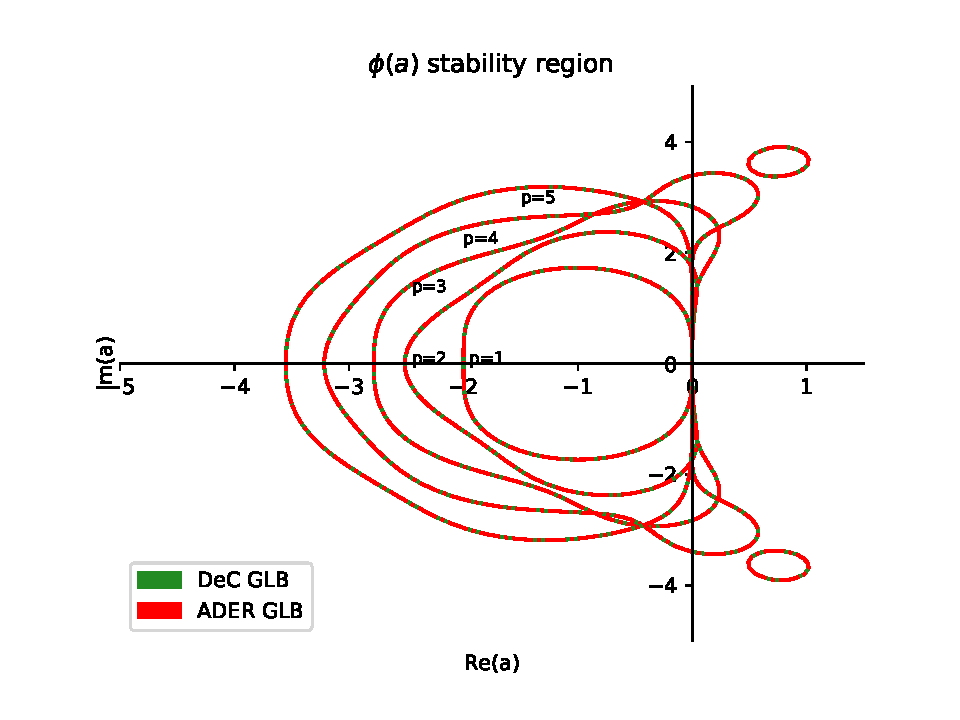
\includegraphics[width=0.45\textwidth, trim={30 20 30 20},clip]{stab_glb.pdf}
    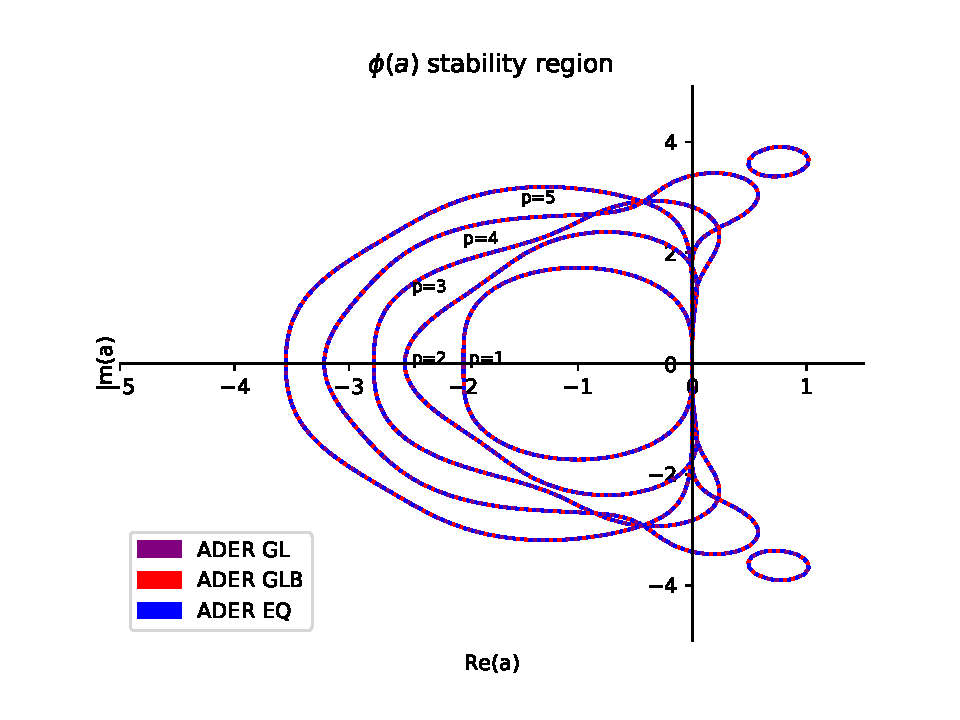
\includegraphics[width=0.45\textwidth, trim={30 20 30 20},clip]{ader_all.pdf}
    \caption{Stability region}
    \label{fig:stab}
\end{figure}

\end{frame}

\begin{frame}{Convergence}

\begin{figure}
\begin{minipage}[c]{0.55\linewidth}
\begin{equation}
\label{eq:scalar-nonlinear}
\begin{split}
&y'(t) = - |y(t)| y(t) ,\\
&y(0) = 1,\\
&t\in [0,0.1].
\end{split}
\end{equation}
Convergence curves for ADER and DeC, varying the approximation order and collocation of nodes for the subtimesteps for a scalar nonlinear ODE 
\end{minipage}
\hfill
\begin{minipage}[c]{0.4\linewidth}
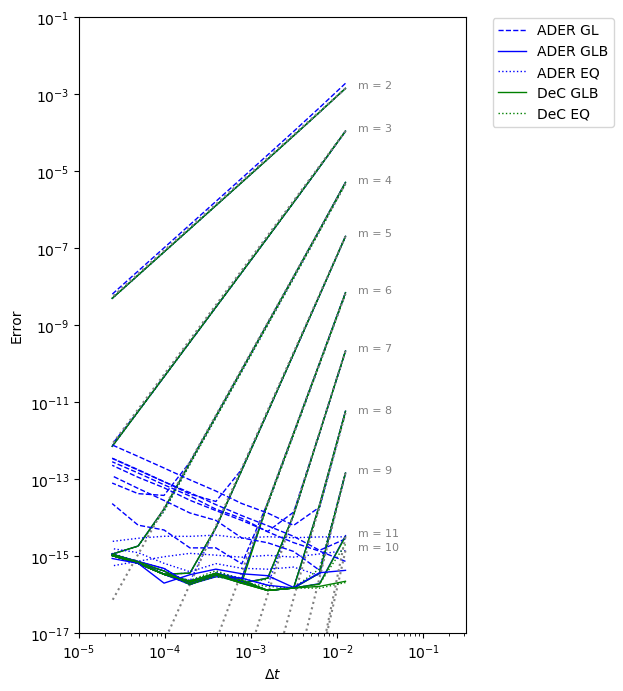
\includegraphics[width=\linewidth]{scalar-2.png}
\end{minipage}%
\end{figure}


\end{frame}

\begin{frame}{Lotka--Volterra}
%\begin{equation}
%\label{eq:system-nonlinear}
%\begin{split}
%y_1'(t) &= \alpha y_1(t) - \beta y_1(t) y_2(t) \\
%y_2'(t) &= -\gamma y_2(t) + \delta y_1(t) y_2(t)
%\end{split}
%\end{equation}
\begin{figure}
	\begin{columns}
	\column{.6\linewidth}
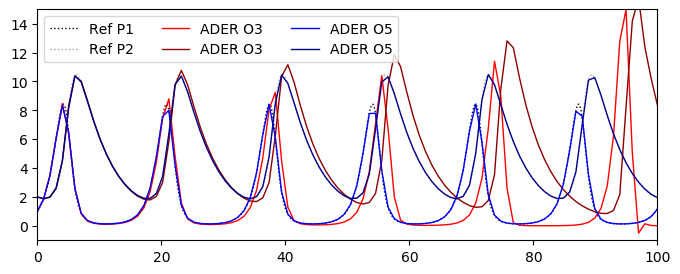
\includegraphics[width=0.95\linewidth]{n100_ader.png}
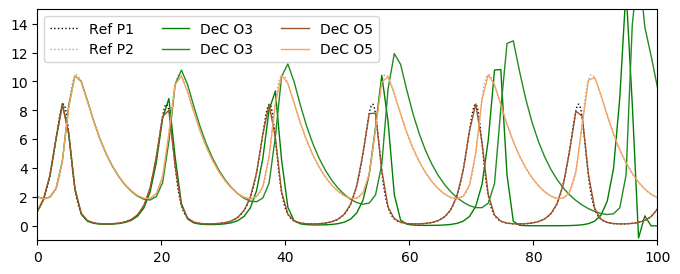
\includegraphics[width=0.95\linewidth]{n100_dec.png}
\column{.3\linewidth}
\caption{Numerical solution of the Lotka-Volterra system using ADER (top) and DeC (bottom) with Gauss-Lobatto nodes with timestep $\Delta T = 1$. \label{fig:lodka-sol-dec}}
\end{columns}
\end{figure}

\end{frame}

\begin{frame}{PDE: Burgers with spectral difference}
\begin{figure}
\begin{center}
	\begin{columns}
		\column{0.35\linewidth}
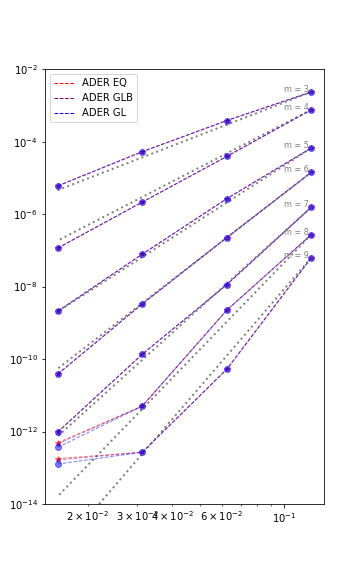
\includegraphics[width=\linewidth,trim={0 55 0 60},clip]{burgers_temp_ader.png}
		\column{0.35\linewidth}
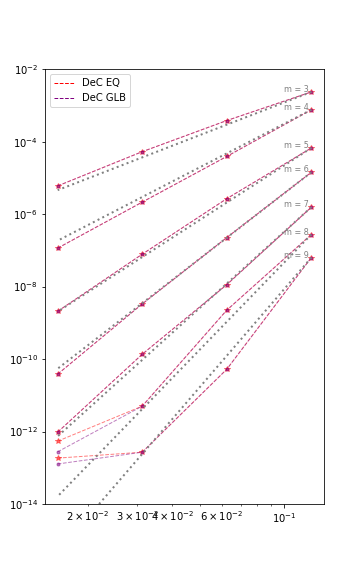
\includegraphics[width=\linewidth,trim={0 55 0 60},clip]{burgers_temp_dec.png}
		\column{0.25\linewidth}
\caption{Convergence error for Burgers equations: Left ADER right DeC. Space discretization with spectral difference}
\label{fig:advection-conv-dec}
	\end{columns}
\end{center}
\end{figure}

\end{frame}


\end{document}




